\documentclass[sigconf]{acmart}
% Cleaning 
\pagestyle{fancy} % removes running headers
\settopmatter{printacmref=false} % Removes citation information below abstract
\renewcommand\footnotetextcopyrightpermission[1]{} % removes footnote with conference information in first column
\pagestyle{plain} % removes running headers
\fancyhead{}
\settopmatter{printacmref=false, printfolios=false}
% Copyright
\setcopyright{none}
% \setcopyright{acmcopyright}
% \setcopyright{acmlicensed}
% \setcopyright{rightsretained}
% \setcopyright{usgov}
% \setcopyright{usgovmixed}
% \setcopyright{cagov}
% \setcopyright{cagovmixed}
\settopmatter{printacmref=false} % Removes citation information below abstract
\acmDOI{}

\usepackage{booktabs} % For formal tables
\usepackage{url}
\usepackage{algorithm}
\usepackage{tabularx}
\usepackage[noend]{algpseudocode}
\algtext*{EndWhile}% Remove "end while" text
\algtext*{EndIf}% Remove "end if" text
%\usepackage{flexisym}

\setlength{\parskip}{0pt}
\setlength{\parsep}{0pt}
\setlength{\headsep}{0pt}
\setlength{\topskip}{0pt}
\setlength{\topmargin}{0pt}
\setlength{\topsep}{0pt}
\setlength{\partopsep}{0pt}
%\linespread{0.95}
\usepackage{mdwlist}
\usepackage{amsmath}

\begin{document}
\title{Query refinement: type aware approach}
\titlenote{https://github.com/ZahraTaherikhonakdar/Eval-QR-type-aware-approach}
\author{Zahra Taherikhonakdar}
\affiliation{
  \institution{University of Windsor}
%   \streetaddress{P.O. Box 1212}
%   \city{Toronto} 
%   \state{ON} 
%   \country{Canada} 
%   \postcode{43017-6221}
}
\email{taherik@uwindsor.ca}
\author{Aaditya Pradipbhai Parekh}
% \authornotemark[1]
\orcid{0000-0002-6033-6564}
\affiliation{
 \institution{University of Windsor}
%   \city{Fredericton} 
%   \state{NB} 
%   \country{Canada} 
}\email{parekh23@uwindsor.ca}

\begin{abstract}
The goal of this research is to improve query refinement considering query types. In general, in the proposed method, the TREC2009 Million Query dataset \cite{WinNT} is used as the input of the ReQue \cite{tamannaee2020reque} to investigate the different query expanders' performance given different query types. In this report, we present the results of the proposed method evaluation.
\end{abstract}

\keywords{Query Refinement, Query Types, Information retrieval}
\maketitle


\section{EXPERIMENTAL SETUP AND EVALUATION}
\subsection{Dataset}
In our experiments, we use a publicly available TREC 2009 Million Query Track \cite{WinNT}. It consists of approximately 40,000 queries collected from a large search log. About 400 queries out of 40,000 queries were categorized into the following query types: navigational, informational-close, informational-open, resource, and advice. The aim of navigational queries is to find a specific URL. Queries which categorized into informational-close and informational-open categories. Their aim is to find the direct (unambiguous) information and undirect information (seek all available information about the topic), respectively. Queries in the resource category are also called transnational queries with the aim of, for example, downloading music from a website. Advice queries find the ideas regarding a general question \cite{carterette2009million}. 

\subsection{Setup}
The main part of the methods is done by ReQue \cite{tamannaee2020reque}. The ReQue is a tool to examine different expander methods on the input queries and generate refined queries which improve the information retrieval task. The whole experiment consists of two steps:  

\subsubsection{Preprocess input data}
In this step, we preprocess the TREC2009 Million Query dataset and its relevance judgment to be accepted as an input for the ReQue.

\subsubsection{Running the ReQue}
In this step, we run the ReQue on the preprocessed dataset. The ReQue requires three inputs: 1- the datasets of queries and their relevance judgments. 2- an information retrieval method which in this experiment, we select the BM25 method. 3- an evaluation metric which MAP is chosen for this experiment. The results of the ReQue would be refinements of initial queries which enhance the performance of the information retrieval task and the expanders which produce these refined queries. We use Tagmee, Glove, and LovinsStemmer as query expanders methods in ReQue.

\subsection{Metrics}
As the performance of the information retrieval task with trec2009 data set is run and evaluated by the ReQue, we set the ReQue to use BM25 \cite{enwiki:1082128332} as an information retrieval task and use MAP (mean average precision) \cite{enwiki:1077036698} as our evaluation metric.
\subsection{Evaluation}
In this section, we evaluate the results based on the specified query types. We build a matrix of query expanders and query types and add one if the expander improves the query in specific query types. For instance, if the Tagmee expander method could improve the input query in navigational query type, we add one value to the specific cell based on each improvement. 

Table 1 contains the example of refined queries by given query expanders.

\begin{table}[h]
\begin{tabularx}{0.43\textwidth} { 
  | >{\raggedright\arraybackslash}X 
  | >{\centering\arraybackslash}X 
  | >{\centering\arraybackslash}X
  | >{\raggedright\arraybackslash}X | }
 \hline
Query Expander & Initial Query & Refined Query \\
 \hline
Tagmee  & cuttle fish bone & cuttle fish bone Cuttlefish \\
 \hline
Glove  & premedication for dental procedures & premedication dentists dentistry required\\
\hline 
Lovins  & pinecrest tropical gardens & pinecrest trop garden\\
\hline
\end{tabularx}
\caption{\label{tab:table-name}Refined queries by different query expanders }
\end{table}

Figure 1 shows the matrix. Columns C1, C2, and C3 represent Tagmee, Glove, and Lovins expanders, respectively. Rows 1, 2, 3, 4, and 5 represent informational-close, informational-open, navigational, resource, and advice, respectively.

\begin{figure}[h]
\centering
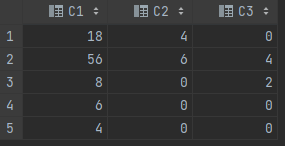
\includegraphics[width=0.8\columnwidth]{Images/matrix.png}
\caption{The Matrix.\label{neural_net}}
\end{figure}

In this experiment, we have 78 informational-close, 213 informational-open, 59 navigational, 42 resource, and 14 advice queries. 

For better representation of the results, we draw the heat-map of the given matrix. Figure 2 shows the heat map.

\begin{figure}[h]
\centering
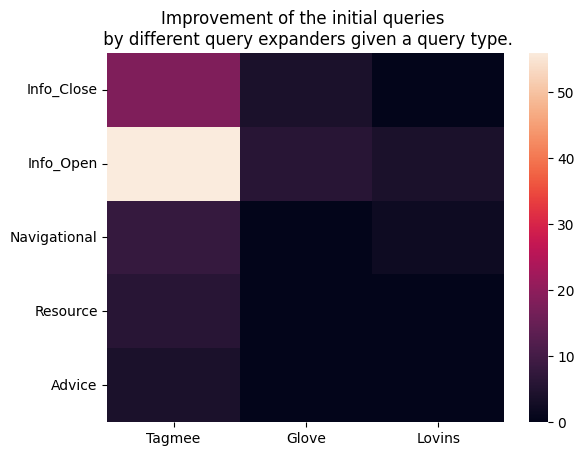
\includegraphics[width=0.8\columnwidth]{Images/heatmap.png}
\caption{The Heat Map.\label{neural_net}}
\end{figure}



As figure 1 and figure 2 show, Tagmee improves all query types but improves informational-open queries the most. The Glove only improves informational-open and informational close, respectively. The Lovins improves informational-open and navigational queries. All query types improve most by the Tagmee expander.

Zero in each cell means that the expander could not improve any query in the specific query type or that query type could not be improved by the specific query expander. For instance, quires in the advice type could not be improved by the Glove expander, or the Lovins could not improve the queries in the informational-close type.

One reason that fewer or zero queries in navigational, resource, and advice categories could be improved by given query expanders could the fewer quantity of them are exist in the input. 

For future work, we are going to have more quires of each type and examine more query expanders to come up with comprehensive and reliable results.
\newpage


\bibliographystyle{ACM-Reference-Format}
\bibliography{bibliography.bib} 

\end{document}

